\chapter*{Đặt vấn đề}\label{chap0}
\addcontentsline{toc}{chapter}{Đặt vấn đề}
% \vspace{5mm}
% \begin{figure}[h]
% 	\begin{tabular}{cc}
% 		\begin{minipage}[b]{0.5\textwidth}
% 			\begin{lstlisting}[language=C++]
% class B {
% 	int b;
% 	int stub(int x); // ERROR
% }
% int foo(B param) {
% 	if (param.b == 1) {
% 		int ret = param.stub(b);
% 		if (param.b == 2) 
% 		return ret;
% 	}
% 	return 0; 
% }  
% 			\end{lstlisting}
% 		\end{minipage}
% 		& \begin{minipage}[b]{0.5\textwidth}
% 			\centering
% 			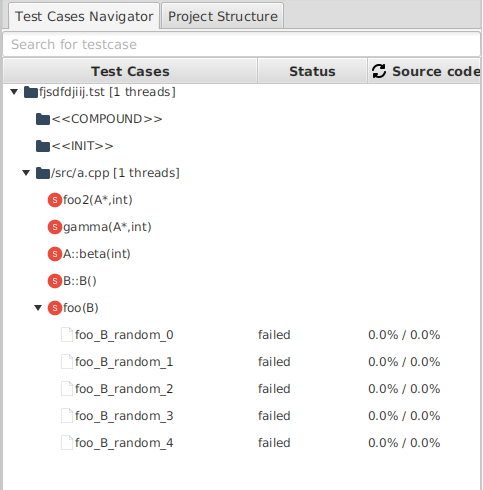
\includegraphics[width=\linewidth]{images/effect.png}
% 		\end{minipage}
% 	\end{tabular}
% 	\caption{Ví dụ sự ảnh hưởng của hàm thiếu định nghĩa khi kiểm thử đơn vị tự động.}
% 	\label{fig:affect}
% \end{figure}

Hiện nay, trong thời đại chuyển đối số khi mà mọi giao dịch, thanh toán đều được thực hiện trên thiết bị di động của người dùng, các nhà phát triển phần mềm đứng trước một cơ hội để tối ưu hóa các quy trình rườm rà đã có nhằm giảm thiểu tương tác trực tiếp giữa nhà cung cấp dịch vụ và người dùng từ đó đẩy nhanh quy trình nghiệp vụ.
Một trong các lĩnh vực được quan tâm và chuyển đổi mạnh mẽ trong những năm gần đây đó là về lĩnh vực dịch vụ ăn uống tại Việt Nam.
Trong đại dịch Covid-19, đã có một sự dịch chuyển lớn trong ngành ẩm thực.
Năm 2020, một khảo sát đã chỉ ra rằng số lượng người đến ăn tại nhà hàng đã giảm trên 90\% do lệnh phong tỏa của các quốc gia và nỗi sợ nguy cơ lây nhiễm từ người qua người~\cite{dube2021covid}.

\begin{figure}[ht]
	\centering
	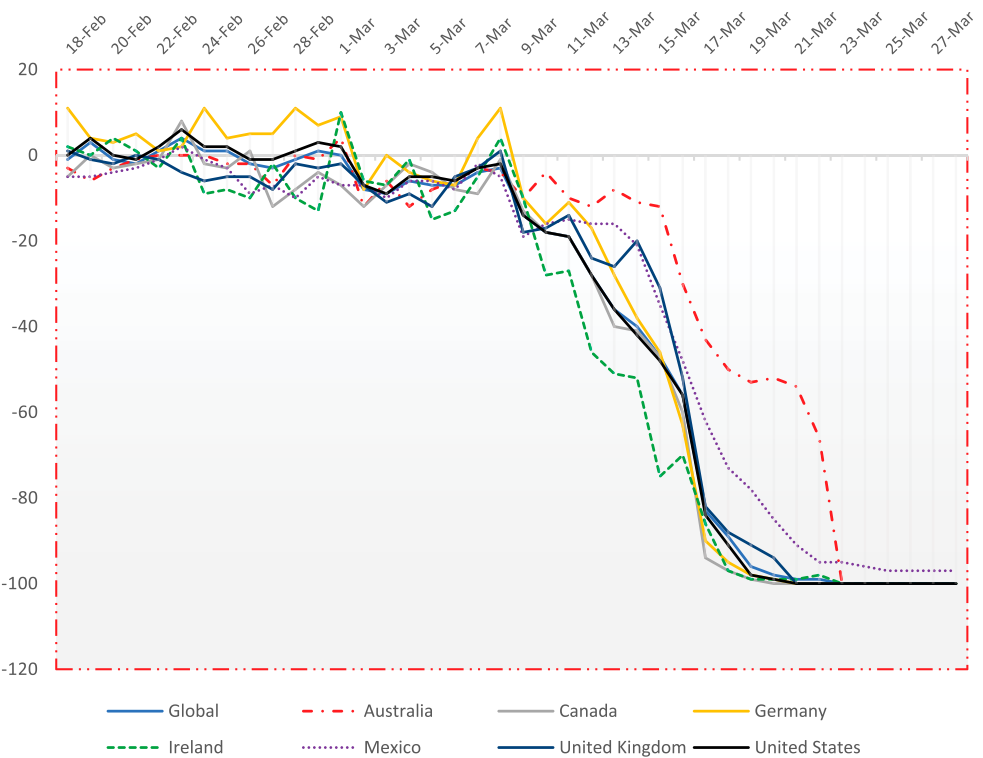
\includegraphics[width=\textwidth]{images/hChip/state-of-global-restaurant-industry-2020.png}
	\caption{Số liệu khách đến nhà hàng tại các nơi trên thế giới~\cite{dube2021covid}}
	\label{fig:state-of-global-restaurant-industry-2020}
\end{figure}

Mặc dù các ứng dụng đặt đồ ăn trực tuyến đã tồn tại từ lâu từ trước khi đại dịch xảy ra, nhưng khi khách hàng không còn lựa chọn ra ngoài ăn, số lượng người dùng mới đăng ký tham gia những nền tảng này tăng đáng kể xuyên suốt thời gian này~\cite{hoang2021customer}.
Các khảo sát sau đó cũng cho thấy rằng 64\%~\cite{pham2020study} người Việt Nam dự định tiếp tục sử dụng các ứng dụng đặt đồ ăn trong tương lai.
Như vậy từ sau đại dịch, đã có sự gia tăng một cách nhanh chóng trong thói quen đặt đồ ăn trực tuyến và mua hàng online của người dùng.
Khảo sát cũng cho thấy người dùng đặt ưu tiên về độ sạch sẽ của nhà hàng lên cao ngoài chất lượng món ăn khi họ đi ăn~\cite{hoang2021customer}.
Từ tất cả những điều trên, các quán ăn, nhà hàng mới chớm nở trong những năm trở lại đây đều gặp phải những trở ngại, thách thức nếu mong muốn mở rộng, phát triển và thu hút khách hàng tiềm năng đến với địa chỉ của họ.
Các quán ăn giờ đây cần phải chuyển dịch cơ cấu bán hàng của họ qua hình thức bán hàng trực tuyến~\cite{matsenko2021transformation}.
Điều này tức là mở rộng độ phủ của họ, tham gia vào các nền tảng bán hàng trực tuyến như Shopee Food, Grab Food, v.v.
Ngoài ra, việc thực khách giờ đây đặt ưu tiên sự sạch sẽ lên cao cũng tạo áp lực cho nhà hàng cần quản lý chặt chẽ nguồn cung của mình.
Đối với các quán ăn nhỏ lẻ, việc phát triển đồng thời hai phương thức bán hàng đó là bán hàng trực tuyến và bán hàng truyền thống rất tốn kém do chi phí đi kèm từ việc tham gia các nền tảng bán hàng trực tuyến đó là phí duy trì thành viên lên tới 25\% cho Shopee Food\footnote{https://merchant.shopeefood.vn/edu/article/phi-mo-gian-hang-va-chiet-khau-tren-shopeefood-la-bao-nhieu}.
Từ đây nhiều quán ăn chọn cách chuyển dịch cơ cấu sang chỉ buôn bán online nhằm giảm thiểu tối đa chi phí phát sinh cho việc thuê mặt bằng, chỗ ngồi cho khách hàng cũng như là chi phí cho các ứng dụng, hệ thống quản lý quán ăn.

Ý tưởng về một ứng dụng quản lý nhà hàng đã được thị trường đón nhận và triển khai rộng rãi trong nhiều năm trở lại đây.
Các giải pháp như Sapo FnB (Food and Beverage) hay KiotViet là một trong các ứng dụng tiên phong trong việc hỗ trợ quản lý hoạt động kinh doanh của nhà hàng.
Tuy nhiên, các ứng này thường chỉ tập trung vào quản lý nội bộ mà chưa thực sự tận dụng được những tiềm năng khi kết nối giữa nhà hàng với khách hàng, còn thiếu tính năng giúp tương tác và chia sẻ thông tin giữa nhà hàng và khách hàng, cũng như khả năng tiếp cận và thu hút khách hàng tiềm năng.
Bằng việc thúc đẩy tương tác giữa thực khách và nhà hàng, chủ cửa hàng sẽ có cái nhìn tổng quát hơn về doanh thu, tình trạng làm ăn của cửa hàng.
Từ đó, nhà hàng và quán ăn có thể đưa ra những chính sách hỗ trợ tốt hơn cho các khách hàng tiềm năng, giúp tương tác với khách hàng tốt hơn.

Khóa luận này trình bày về quá trình phát triển một giải pháp, một hệ thống hỗ trợ quản lý nhà hàng, quán ăn cho các thành viên tham gia sử dụng.
Nền tảng quản lý nhà hàng, quán ăn, cung cấp một ứng dụng cho phép các nhà hàng quản lý quán ăn của họ bao gồm quản lý nhân viên, thực đơn, thống kê doanh thu, hóa đơn theo các mốc thời gian cụ thể.
Ngoài ra nền tảng còn cung cấp giải pháp giúp các bên tham gia xây dựng nên một trang giới thiệu cho chính nhà hàng của họ đi kèm các dịch vụ như đặt bàn, hỗ trợ khách hàng, v.v.
Trong tương lai, hệ thống cũng hướng đến việc cho phép người dùng tạo lập tài khoản cho chính họ và cung cấp các tính năng giúp người dùng quản lý những thông tin như lịch sử ăn tại những nhà hàng, quán ăn họ đã đến và tìm kiếm các quán ăn dựa theo khẩu vị, địa điểm của người dùng.
Một khi người dùng đã có tài khoản trên nền tảng, các quán ăn, nhà hàng có thể biết được thông tin của người đến ăn nếu họ có trong hệ thống, từ đó đưa ra các chương trình khuyến mãi hợp lý cho bất kỳ thực khách quen nào tại chuỗi nhà hàng, quán ăn đó.

Để đáp ứng được đầy đủ các chức năng nghiệp vụ được đặt ra với số lượng người dùng lớn từ các nhà hàng, quán ăn trải dài khắp cả nước, hệ thống của nền tảng quản lý nhà hàng, quán ăn cần đáp ứng số lượng người dùng lớn, đặt biệt trong những khung giờ cao điểm.
Khả năng dễ dàng mở rộng về mặt phần cứng  cũng là một yếu tố quan trọng được chú ý đến khi nền tảng tận dụng khả năng mở rộng hệ thống tự động của GKE (Google Kubernetes Engine) thông qua tính năng autoscale (tự động mở rộng) khi hệ thống trải qua một lượng truy cập lớn.
Chi tiết về thiết kế của hệ thống sẽ được nói rõ hơn trong Chương~\nameref{chap2}

Phần còn lại của khóa luận được trình bày như sau.
Chương~\ref{chap1} trình bày giới thiệu về thiết kế tổng quan của hệ thống và các chức năng chính cũng như đi qua biểu đồ ca sử dụng của một vài chức năng cụ thể.
Tiếp theo, Chương~\ref{chap2} mô tả chi tiết thêm về từng thành phần cấu thành hệ thống, từ thiết kế của các cơ sở dữ liệu cho đến luồng người dùng cho nhà hàng, quán ăn, khách hàng, v.v.
Chương~\ref{chap3} sẽ giới thiệu về các công nghệ được sử dụng trong quá trình xây dựng hệ thống, chia sẻ về quá trình cài đặt và triển khai hệ thống lên môi trường đám mây của Google, tích hợp CI/CD (Continuous Integration/Continuous Delivery) cho dự án giúp tự động hóa quá trình cài đặt cũng như đảm bảo tính sẵn sàng cao cho hệ thống khi chạy thực nghiệm.
Ngoài ra Chương~\ref{chap3} cũng mô tả luồng kỹ thuật dưới dạng sơ đồ tuần tự khi người dùng thực hiện các chức năng cụ thể trên ứng dụng.
Cuối cùng Chương~\ref{chap4} thực hiện đánh giá hệ thống, hiệu quả hoạt động thông qua các bộ kiểm thử cụ thể cho từng tính năng được chọn.